\section{Ergebnisse}
\label{Ergebnisse}
In diesem Kapitel werden die Ergebnisse der Implementierung vorgestellt. Zunächst werden die zentralen Funktionalitäten der Gruppenfunktion, \ac{HID} und des Massenspeichermediums vorgestellt. Daraufhin werden die Ergebnisse diskutiert und im Abschluss wird der Stand der Produktentwicklung vorgestellt.

\subsection{Evaluierung}

\subsubsection{Massenspeichermedium}
Wird der Fußschalter über \ac{USB} mit einem Computer verbunden, zeigt er sich als ein Massenspeichermedium. In Abbildung \ref{fig:LaufwerkMassenspeichermediums} ist das geöffnete Laufwerk unter Windows mit den zwei Konfigurationsdateien config.ini und devices.csv zu sehen.
\begin{figure}[H] 
	\centering
	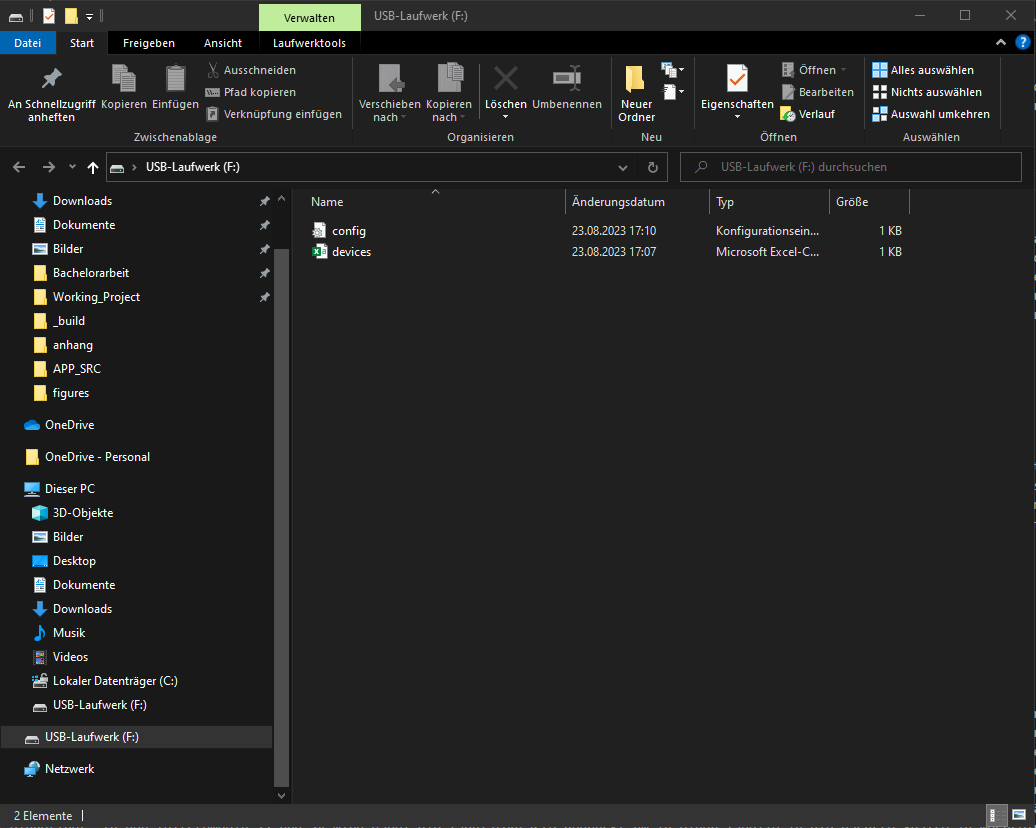
\includegraphics[width=\textwidth]{figures/Laufwerk.png}
	\caption{Laufwerk des Massenspeichermediums}
	\label{fig:LaufwerkMassenspeichermediums}
\end{figure}

In Abbildung \ref{fig:GlobaleKonfigurationsdatei} ist der Inhalt der gobalen Konfigurationsdatei zu sehen. Die Zeilen mit einem ``\#'' am Zeilenanfang kennzeichnen eine Kommentarzeile und werden nicht eingelesen. Der Anwender kann die Datei um eigene Kommentare erweitern, muss jedoch aufpassen die maximale Anzahl an erlaubten Zeichen nicht zu überschreiten. Es beeinhaltet die Einstellungsmöglichkeiten des Messmodus und des Protokolls das über den virtuellen COM-Port gesprochen wird. Mit der ``KeyboardLanguageID'' kann der Fußschalter auch in den, im Kommentar, angegebenen Ländern eingesetzt werden. Mit dem Einstellungsmöglichkeiten des ``value seperator'', ``data set seperator'' und ``number seperator'' kann die Ausgabe des Messergebnis über \ac{HID} konfiguriert werden. Das Attribut ``key\_single\_press'' gibt an, welches Zeichen bei einem einfachen Klick in den Modi 0 und 4 vom Fußschalter übertragen wird. Dementsprechend gibt ``key\_double\_press'' an, welches Zeichen bei einem Doppelklick ausgegeben wird. Mit dem Attribut ``InactivityTimeout'' kann der Anwender einstellen, nach welcher Zeitdauer der Innaktivität in Sekunden der Fußschalter sich ausschaltet. Das letzte Attribut das gesetzt werden kann, ist ``sequentialGroup''. Es gibt an ob die Messergebnisse einer Gruppenmessungen alle zusammen ausgegeben werden oder ob bei jeder Betätigung des Fußtasters jeweils das nächste Messergebnis abgefragt wird.
\begin{figure}[H] 
	\centering
	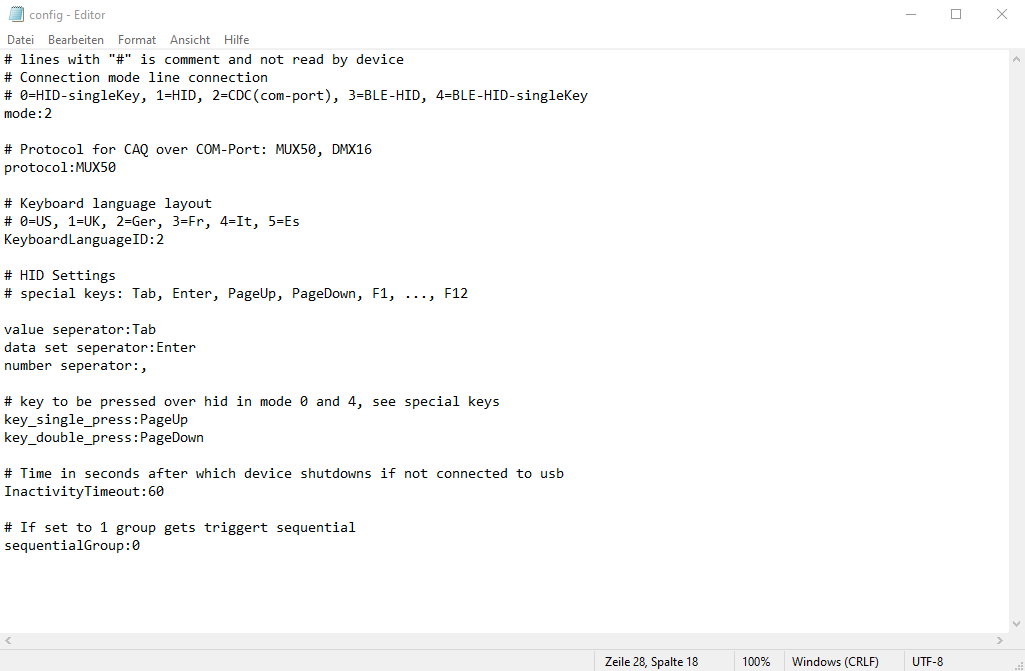
\includegraphics[width=\textwidth]{figures/configfile.png}
	\caption{Globale Konfigurationsdatei}
	\label{fig:GlobaleKonfigurationsdatei}
\end{figure}

In Abbildung \ref{fig:KonfigurationsdateiWerkzeuge} ist die Konfigurationsdatei zu sehen, in der angegeben werden kann, mit welchen Werkzeugen der Fußschalter sich verbindet. Mit einer Null in der ``Activ'' Spalte wird ein Gerät aus der Suche des Fußschalters ausgenommen. Damit der Fußschalter ein Werkzeug finden kann, müssen Name und Seriennummer zwingend korrekt sein. Die Einträge ``Channel'' und ``Angle Channel'' werden für die Kommunikation mit der \ac{CAQ}-Software benötigt, während die Nummerierung in der Spalte ``Group'' die Teilnahme beziehungsweise der Reihenfolge der Gruppe festlegen. Während die Grupppenfunktion auf Messuhren ausgelegt ist, können auch andere Geräte hier eingetragen werden und es treten keine größeren Fehler auf, da die Abfrage des derzeitigen Messergebnis von allen Geräten unterstützt wird.
\begin{figure}[H] 
	\centering
	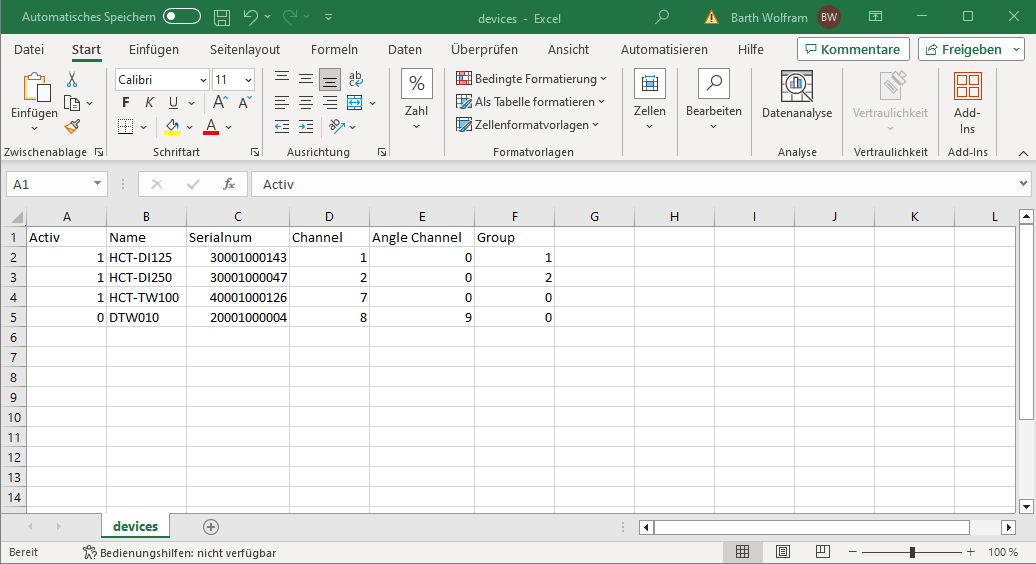
\includegraphics[width=\textwidth]{figures/devicesDatei.png}
	\caption{Konfigurationsdatei der zu verbindenden Werkzeuge}
	\label{fig:KonfigurationsdateiWerkzeuge}
\end{figure}

\subsubsection{Gruppenfunktion}
Bei der Gruppenfunktion ist die größte Herausforderung der Implementierung, dass gerade in den HID Modi die Reihenfolge der Gruppe eingehalten werden muss damit die Messergebnisse in der Ausgabe wieder einem Werkzeug zuordbar sind. In Abbildung \ref{fig:MessungenGruppenfunktionCDC} ist die Ausgabe der Gruppenfunktion über den virtuelle COM-Port im Modus \ac{CDC} zu sehen. Die Ausgabe wird in Terminalprogramm RealTerm aufgefangen und die einzelnen Ausgaben der Gruppenfunktion durch rote Striche getrennt. Durch Betätigen des Fußtasters werden also jeweils die drei Zeilen zwischen den roten Strichen ausgegeben. Durch die Kanalnummern, die nur in diesem Modus Verwendung finden und jeweils am Anfang der Zeilen stehen, sind die Messergebnisse den einzelnen Geräten zuordbar. Zusätzlich wurden die Messuhren auf Messwerte eingestellt, die zu ihren Kanalnummern und Gruppennummern korrespondieren. 
\begin{figure}[H] 
	\centering
	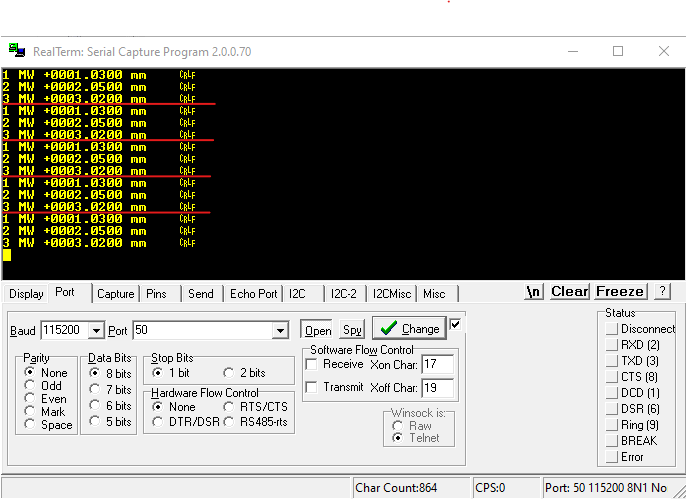
\includegraphics[width=\textwidth]{figures/GroupFeature.png}
	\caption{Durchführung von Messungen mit der Gruppenfunktion über CDC}
	\label{fig:MessungenGruppenfunktionCDC}
\end{figure}

Die gleichen Messungen sind in Abbildung \ref{fig:MessungenGruppenfunktionHID} im Modus \ac{USB}-\ac{HID} durchgeführt. Durch Betätigung des Fußtasters wird jeweils eine Zeile Messwerte ausgegeben. Es ist ersichtlich, dass bei einer Vertauschung der Messergebnisse, bei echten Messdaten, die von Zeile zu Zeile unterschiedlich sind, dies nicht nachvollzogen werden kann. Da hier jedoch die Einhaltung der Reihenfolge gezeigt werden soll, sind die Messergebnisse immer die Gleichen und korrespondieren zu ihren Gruppennummern. Es wird deutlich, dass auch bei mehreren durchgeführten Gruppenmessungen die Reihenfolge der Gruppe eingehalten wird.
\begin{figure}[H] 
	\centering
	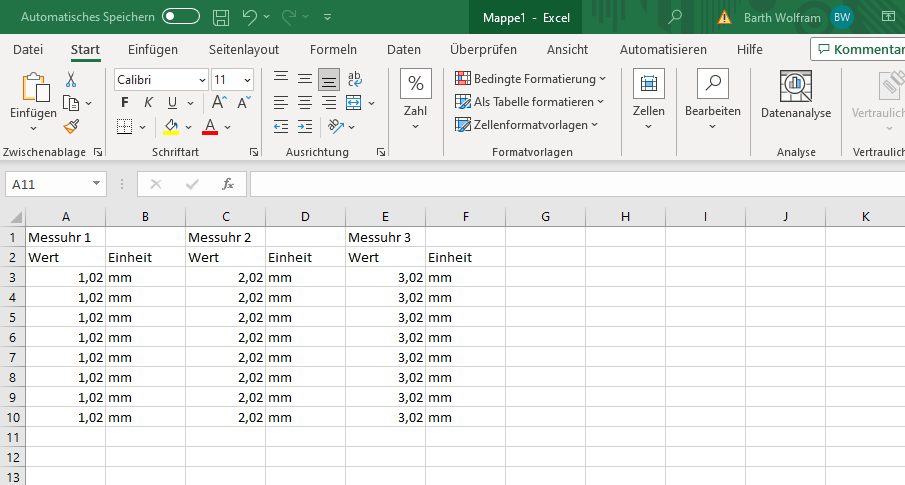
\includegraphics[width=\textwidth]{figures/USBHIDGroup.png}
	\caption{Durchführung von Messungen mit der Gruppenfunktion über HID}
	\label{fig:MessungenGruppenfunktionHID}
\end{figure}

\subsubsection{Zeitmessungen HID}
Für die Modi USB-HID und BLE-HID ist die Zeit die verstreicht bis das gesamte Messergebnis eingetippt wurde das wichtigeste Gütekriterium der Implementierung neben der offentsichtlichen Fehlerfreiheit der Ausgabe. In Abbildung \ref{fig:LoggingAusgabeMessergebnisUSBHID} sind daher die Logausgaben der Aufrufe zur Funktion, welche die einzelnen Tastendrücke an die USB-HID-Library übergibt, zu sehen. In Klammern ist die verstrichene Zeit seit dem ersten Tastendruck in Millisekunden zu sehen. Abgesehen von der Zeitspanne zwischen dem ersten Tastendruck und Tasten loslassen, in der weniger als eine Millisekunde vergangen ist, liegen zwischen jedem einzelnen Aufruf genau zwei Millisekunden. Es ist zu vermuten, dass die Zeitspanne zwischen den ersten beiden Aufrufen niedriger ist, da die Daten noch nicht über USB gesendet wurden, sondern zwischengespeichert sind. Sobald begonnen wird die Daten tatsächlich über USB zu senden, vergehen zwischen zwei Tastendrücken genau zwei Millisekunden. Das Messergebniss wird schnell und gleichmäßig über USB eingetippt. Zu den Zeitstempeln 22 und 24 wird dabei die Tabulatortaste gedrückt um in einer Tabelle in die nächste Spalte zu wechseln, während zum Zeitpunkt 34 und 36 die Zeile terminiert wird und in die nächste Zeile gesprungen wird.
\begin{figure}[H] 
	\centering
	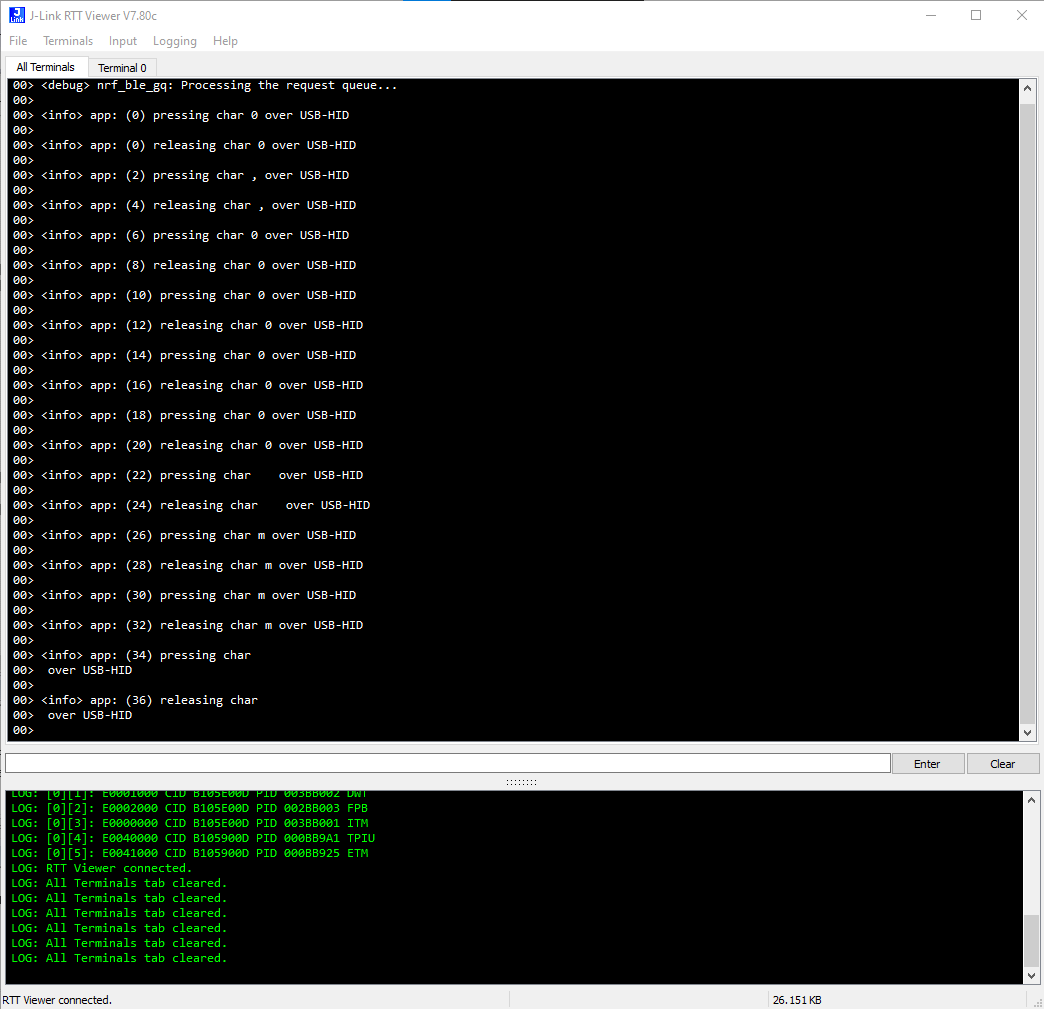
\includegraphics[width=\textwidth]{figures/USBHID.png}
	\caption{Logging einer Ausgabe eines Messergebnis über USB-HID}
	\label{fig:LoggingAusgabeMessergebnisUSBHID}
\end{figure}

Anders ist das zeitliche verhalten bei Eingabe des Messergebnis über BLE-HID. In Abbildung \ref{fig:MitschnittEinerMessuhr} ist der Mitschnitt der BLE-Nachrichten des Fußschalters an den Computer bei einer verbundenen Messuhr zu sehen. Es wurde der Ellisys Bluetooth Analyzer verwendet. Hier ist auch zu sehen wie zum Zeitpunkt 13:30:35.883 das Messergebnis als HCT-Nachricht von der Messuhr an den Fußschalter übertragen wird. Ab dem Zeitpunkt 13:35.948 werden die Tastendrücke vom Fußschalter an den Computer übertragen. Dabei werden die Codes für Tastaturtasten übertragen und nicht die Codes der ASCII-Zeichen. Der Code 0 steht dabei für das loslassen einer Taste. Es wird deutlich, dass die einzelnen Tastendrücke mit unregelmäßigen Abständen eingetippt werden. Die Telegrame zwischen denen weniger als eine Millisekunde verstreicht werden dabei in einem Zeitslot übertragen. Es kommt in unregelmäßigen Zeitabständen dazu, dass mit ungefähr 110 Millisekunden eine im Verhältnis zum Connection Interval lange Zeitspannen zwischen den einzelnen Nachrichten verstreicht, vorallem da das Connection Interval hier 30 Millisekunden beträgt und somit der Fußschalter deutlich mehr Zeitslots für weitere Übertragungen zur Verfügung hätte. Es wird beobachtet, dass die Ausgabe der Zeichen ungleichmäßig ist.
\begin{figure}[H] 
	\centering
	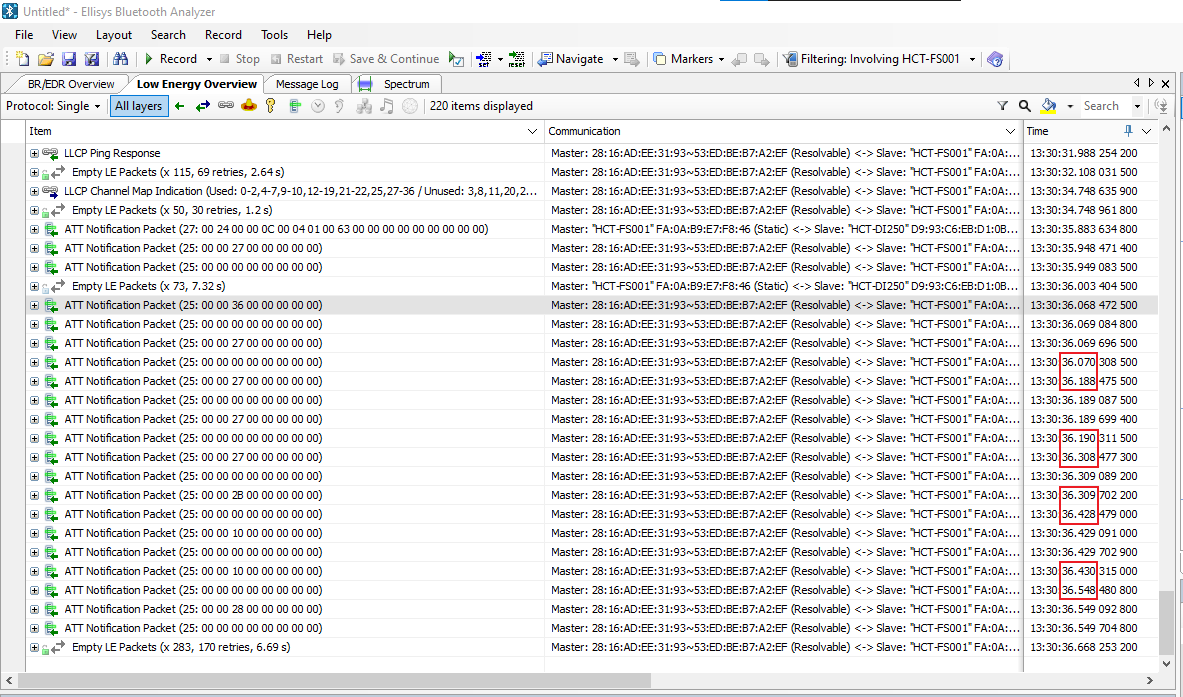
\includegraphics[width=\textwidth]{figures/BLEHID1device.png}
	\caption{Mitschnitt der BLE Nachrichten eines BLE-HID Messergebnis von einer verbundenen Messuhr}
	\label{fig:MitschnittEinerMessuhr}
\end{figure}

Dieses Verhalten verschärft sich, wenn mehrere Messuhren verbunden sind. In Abbildung \ref{fig:MitschnittDreiMessuhr} ist der Mitschnitt der BLE-Nachrichten der Tastendrücke bei drei verbundenen Messuhren zu sehen. Die Übertragungen treten wieder gehäuft auf. In einem Zeitslot werden mehrere Zeichen übertragen zwischen denen weniger als eine Millisekunde verstreicht, während die Zeit bis nur nächsten Übertragung mit 236 Millisekunden fast achtmal so groß wie das Connection Interval von 30 Millisekunden ist. Interessanterweise beträgt die Zeitdauer in allen der drei roten Kästen jeweils exakt 236 Millisekunden.
\begin{figure}[H] 
	\centering
	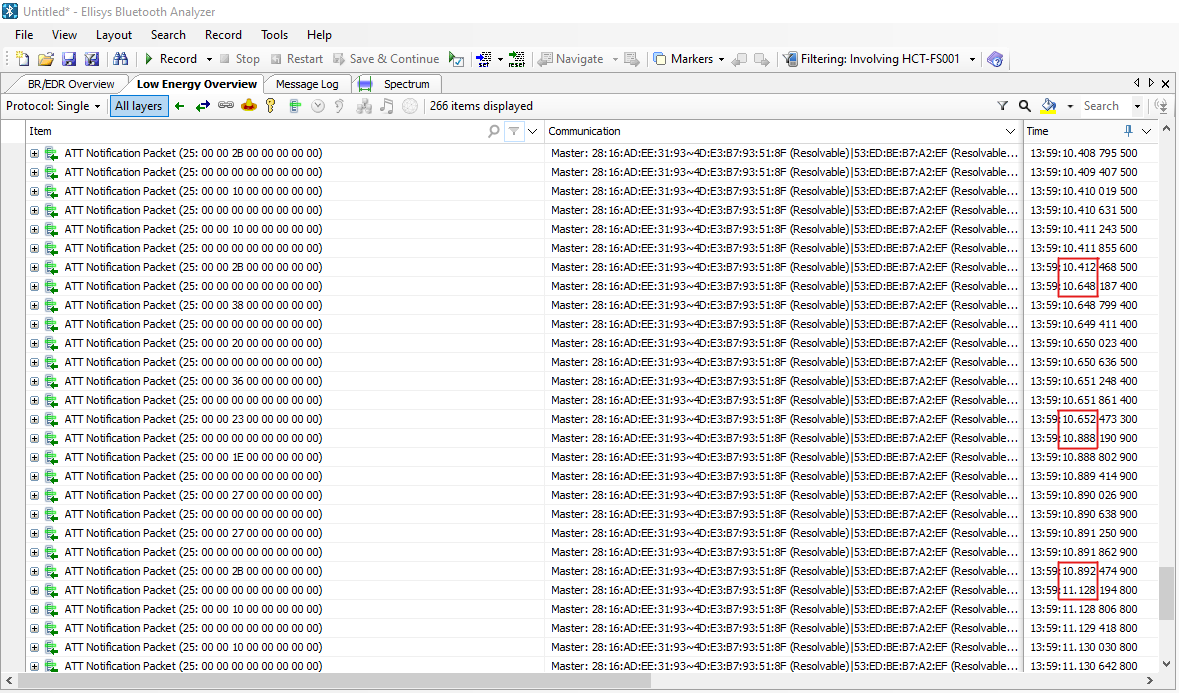
\includegraphics[width=\textwidth]{figures/BLEHID2device.png}
	\caption{Mitschnitt der BLE Nachrichten der BLE-HID Messergebnisse von drei verbundenen Messuhr}
	\label{fig:MitschnittDreiMessuhr}
\end{figure}

Es steht in Verdacht, dass die Connection Intervalle bei mehreren bestehenden Verbindungen nicht gut koordiniert werden. In Abbildung \ref{fig:DiagrammConnectionIntervalle} ist die Aufteilung der Connection Intervalle zu sehen. Dabei ist das untere Gerät mit der MAC-Adresse 28:16:AD:EE:31:93 der Computer mit dem der Fußschalter verbunden ist. Die Pakete seiner Verbindung mit dem Fußschalter sind gleichmäßig im zu erwartenden Abstand des Connection Interval von 30 Millisekunden aufgereiht. Die Pakete der Verbindungen des Fußschalters zu den Messuhren sind ungleichmäßig verteilt. Dabei kommen die Pakete zu den drei Messuhren hintereinander und dann kommt eine Pause. Zudem ist trotz des im Framework definierten und im Verbindungsaufbau ausgehandelten Connection Intervals von 60 Millisekunden ein Connection Interval von 240 Millisekunden zwischen dem Fußschalter und den einzelnen Messuhren zu beobachten. Dabei ist es überraschend weil es relativ genau mit den Verzögerungen in der Ausgabe über HID korreliert. Die Messergebnisse sind jedoch zum Zeitpunkt der Verzögerungen bereits erhalten und es ist derzeit noch unklar wieso der Fußschalter scheinbar ein ganzes Connection Interval zu einer Messuhr mitten in seiner Übertragung der Tastendrücke untätig verstreichen lässt. Dieser Umstand wird derzeit noch analysiert und muss im Rahmen der Produktentwicklung noch optimiert werden.
\begin{figure}[H] 
	\centering
	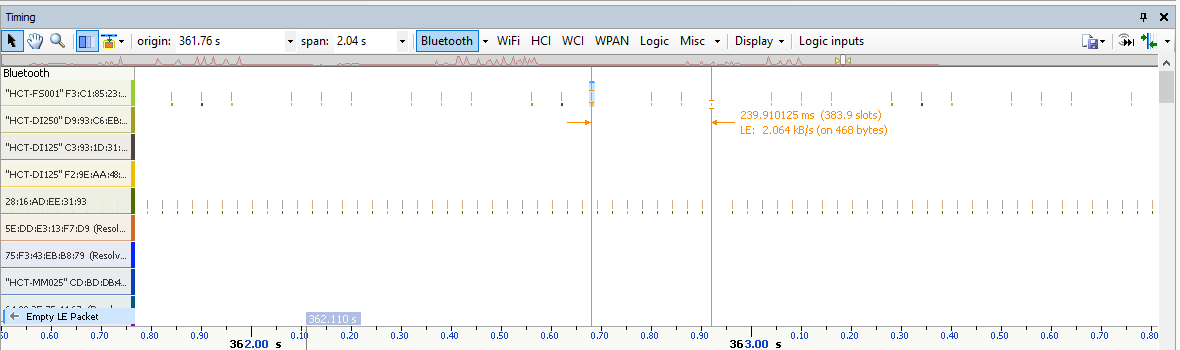
\includegraphics[width=\textwidth]{figures/ConnectionIntervalle.png}
	\caption{Diagramm der Connection Intervalle bei drei Messuhren und einer Verbindung zum Computer}
	\label{fig:DiagrammConnectionIntervalle}
\end{figure}

\subsection{Diskussion}
Für diese Arbeit wurde die Forschungsfrage gestellt, wie die Software- und Hardware-Komponenten eines intelligenten Fußschalters gestaltet werden sollten, damit dieser ohne die Installation weiterer Software Hand- und Messwerkzeug an ein Computersystem kabellose anbindet und deren Messergebisse in verschiedenen konfigurierbaren Formaten zur Verfügung stellt. Es wurde gezeigt, dass ein Gerät entwickelt wurde, dass bis zu Fünf Drehmomentschlüssel oder Messuhren über \ac{BLE} verbinden kann und ihre Messergebnisse über \ac{HID} und \ac{CDC} zur Weiterverarbeitung zur Verfügung stellt. Dadurch werden zwei wichtige Anwendungsfälle abgedeckt. Einerseits die automatisierte Qualitätskontrolle mit einer \ac{CAQ}-Software und anderseits das Auffangen und Speichern der Messergebnisse in einem Texteditor oder Tabellenprogramm. Dabei benötigt es keine weitere Software für Nutzung dieser Funktionalitäten, sondern erfordert lediglich einen Texteditor um die Konfigurationsdateien zu editieren. Lediglich ein Messmodus in dem der Fußschalter zusammen mit der Windows-App agiert steht noch aus, würde jedoch auch für eine unabsehbare Zeit dem Anwender keinen Mehrwert bringen.\\
Es wurde darüber hinausgehend weitere Funktionalitäten wie die Gruppenfunktion entwickelt, welche den Gebrauch von einer größeren Anzahl an Messuhren erleichtert und den Mehrwert des Fußtasters optimiert. Auch eine automatische Detektion der Änderungen der Konfigurationsdateien wurde implementiert um die Umkonfiguration des Fußschalters dem Anwender zu erleichtern und ein Energiemanagement wurde geschaffen um eine maximale Laufzeit zu erreichen, wenn der Fußschalter selbst als ein drahtloses Gerät agiert.\\
Die Forschungsfrage wurde also nicht nur vollständig beantwortet, sondern auch darüberhinausgehende Frage- und Problemstellungen gelöst.


\subsection{Stand Produktvorentwicklung}
Der Fußschalter und der Dongle sollen als eigenständige Produkte in das Sortiment der Hoffmann Group übernommen werden. Für sie werden jeweils Projekte vom Produktmanagement eröffnet. Dabei werden die Hardwareänderungen wie in Kapitel \ref{EnergieManagement} beschrieben, in das Layout der Platine übernommen. Zusätzlich sollen die Pins, die den Chip in den Bootloader Mode versetzt, durch eine Taste von außen erreichbar gemacht werden. Außerdem sollen auch die SWE-Pads, die das Debugging auf dem Chip ermöglichen, erreichbar gemacht werden. Derzeitig sind sie auf der Seite mit der der Dongle auf die Platine gelötet wurde, weswegen sie nur sehr schwer abgreifbar sind. Die Prototypen dieser neuen Hardwareversion sind gegen Ende dieser Arbeit erhalten worden und es wurde bereits festgestellt, dass die Taste die den Fußschalter in den Bootloadermodus versetzt nicht wie spezifiert funktioniert. Der Zulieferer der Platine muss diese daher erneut überarbeiten. Des weiteren werden umfassende Funk- und Reichweitenmessungen durchgeführt, da die ursprüngliche Platine dort nicht die Anforderungen erfüllte.\\
Der Modus \ac{BLE}-Windows-App wurde auf eine spätere Version verschoben, da die Integration der Messuhren und Messschieber in die Windows App andauert, sowie neue Geräte auf den Markt kommen sollen und deren Integration priorisiert wird. Eine Integration des Fußschalters ist daher noch nicht absehbar. Daher wurde die Implementierung des Modus zugunsten anderer Features bis auf Weiteres verschoben.\\
Insbesonders der Dongle ist bereits zu ersten Testläufen an ausgewählte Kunden gegeben worden und hat sich dort bereits bewährt. Desweiteren werden Codereviews mit anderen Entwicklern der Hoffmann Group durchgeführt.\\
Für die Funktionalität des Fußschalter beziehungsweise des Dongles wird eine Erfindungsmeldung herausgegeben und der Prozess der Patentierung der Technik wurde angestoßen. Siehe Anhang \ref{appendix:Erfindungsmeldung}.
